\section{Results (Arc II): A Permutation-Invariant Policy}
\label{sec:relational}

Section~\ref{sec:diagnostic} showed that the flat-MLP DQN's boundary-hugging
traces back to having no inductive bias for treating the sensor field as an
unordered set. The Relational-RL policy in Section~\ref{sec:relational_method}
was designed to address this: a permutation-invariant Deep-Sets encoder trained
with PPO on the same environment and curriculum. The boundary-occupancy diagnostic from Section~\ref{sec:diagnostic} is re-run on
the new policy below, followed by the five-condition head-to-head comparison and
a statement of what the comparison does and does not establish.

\subsection{Boundary-occupancy diagnostic}
\label{sec:relational_diagnostic}

The diagnostic of Section~\ref{sec:diagnostic} is re-run on the Relational-RL
policy under identical conditions: 20 seeds, $200{\times}200$ grid, $N{=}20$,
deterministic action selection (\texttt{argmax} over logits). Results are
reported alongside the DQN in Table~\ref{tab:boundary_compare}.

\begin{figure}[H]
\centering
\includegraphics[width=0.95\linewidth]{../src/agents/dqn/dqn_evaluation_results/baseline_results/boundary_heatmap_compare.png}
\caption{Position-occupancy heatmaps aggregated over 20 seeds, $200{\times}200$
grid, $N{=}20$. (a) The flat-MLP DQN concentrates all flight time on the
grid perimeter. (b) The permutation-invariant Relational-RL policy
distributes flight time across the interior of the grid, retaining a
modest perimeter component near boundary-adjacent sensors.}
\label{fig:boundary_heatmap_compare}
\end{figure}

\begin{table}[H]
\centering
\caption{Boundary-occupancy diagnostic: flat-MLP DQN vs Relational-RL policy, 20 seeds, $200{\times}200$ grid, $N{=}20$.}
\label{tab:boundary_compare}
\begin{tabular}{lcc}
\toprule
\textbf{Metric}                          & \textbf{DQN (flat MLP)} & \textbf{Relational RL (PPO)} \\
\midrule
\texttt{boundary\_hits} (mean)           & 21.8            & \textbf{0.00}              \\
\texttt{boundary\_hits} (max)            & 267             & \textbf{0}                 \\
\texttt{edge\_step\_pct} (mean)          & 100.0\%         & \textbf{21.5\%}            \\
\texttt{edge\_step\_pct} (median)        & 100.0\%         & \textbf{22.9\%}            \\
Full-coverage episodes (cov. $= 100\%$)  & 15 / 20         & \textbf{20 / 20}           \\
\bottomrule
\end{tabular}
\end{table}

Most visibly, the perimeter-adjacent pathology is eliminated. Mean edge-cell occupancy falls from $100\%$ to $21.5\%$. The Relational-RL
policy spends roughly four-fifths of every episode in the grid interior.
This is not a marginal shift: it is the complete inversion of the dominant
spatial behaviour, with no change to the reward function, environment
physics, or curriculum.

Wall-collision counts confirm this. The Relational-RL policy records zero failed moves across all twenty seeds.
The DQN's wall-collision rate has a heavy right tail (three seeds with
$3, 165, 267$ hits respectively) consistent with occasional collapse onto
an infeasible monotone action; no such failure mode appears in the new
architecture.

Coverage tells the same story. Every Relational-RL episode achieves $100\%$ sensor coverage; the DQN
achieves this on $15$ of $20$ episodes. The five DQN failures are precisely
the seed conditions identified in Section~\ref{sec:diagnostic} on which the
perimeter-adjacent trajectory cannot reach every sensor within the battery
horizon.

\subsection{Head-to-head performance}
\label{sec:relational_headtohead}

\begin{figure}[H]
\centering
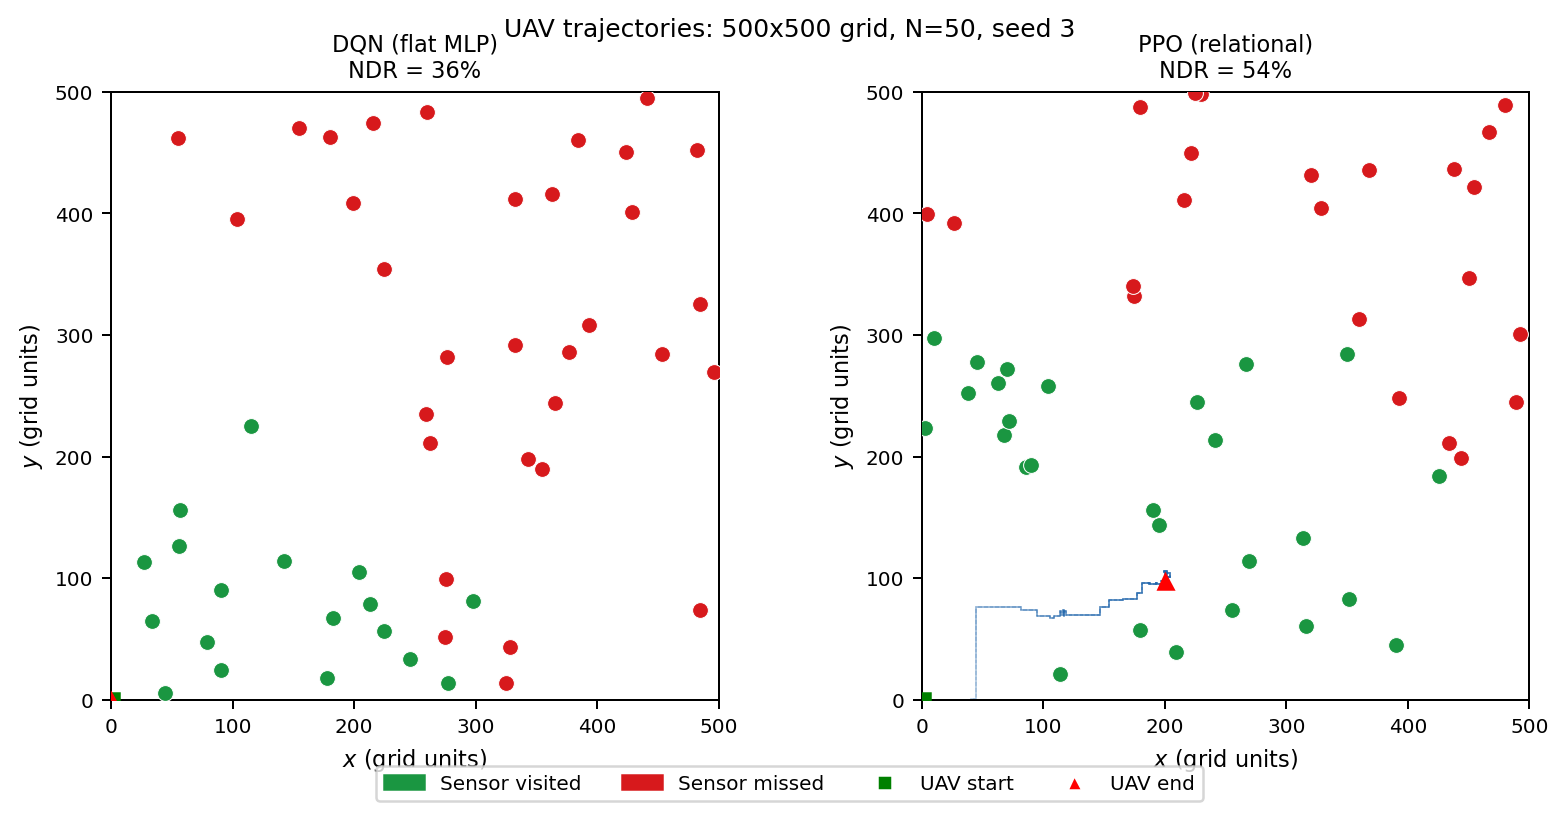
\includegraphics[width=\linewidth]{../src/agents/dqn/dqn_evaluation_results/baseline_results/trajectory_dqn_vs_relational.png}
\caption{UAV trajectories for one representative episode at $500{\times}500$, $N{=}50$ (seed 3). Green circles are sensors from which data was collected; red circles were not reached. The DQN stays near the origin for the full episode, collecting only the sensors within its immediate LoRa range. The relational policy moves through the grid and reaches sensors scattered across the deployment area. Aggregate NDR across 50 seeds is reported in Table~\ref{tab:scalability_ndr}.}
\label{fig:trajectory_compare}
\end{figure}

Figure~\ref{fig:scalability_combined} and Table~\ref{tab:scalability_ndr} summarise the comparison across five $(\text{grid}, N)$ conditions. Seed-matched bootstrap confidence intervals on the three diagnostic metrics at $200{\times}200$, $N{=}20$ are in Figure~\ref{fig:dqn_vs_rel_forest} (Appendix~\ref{app:extended_results}).

\begin{figure}[H]
\centering
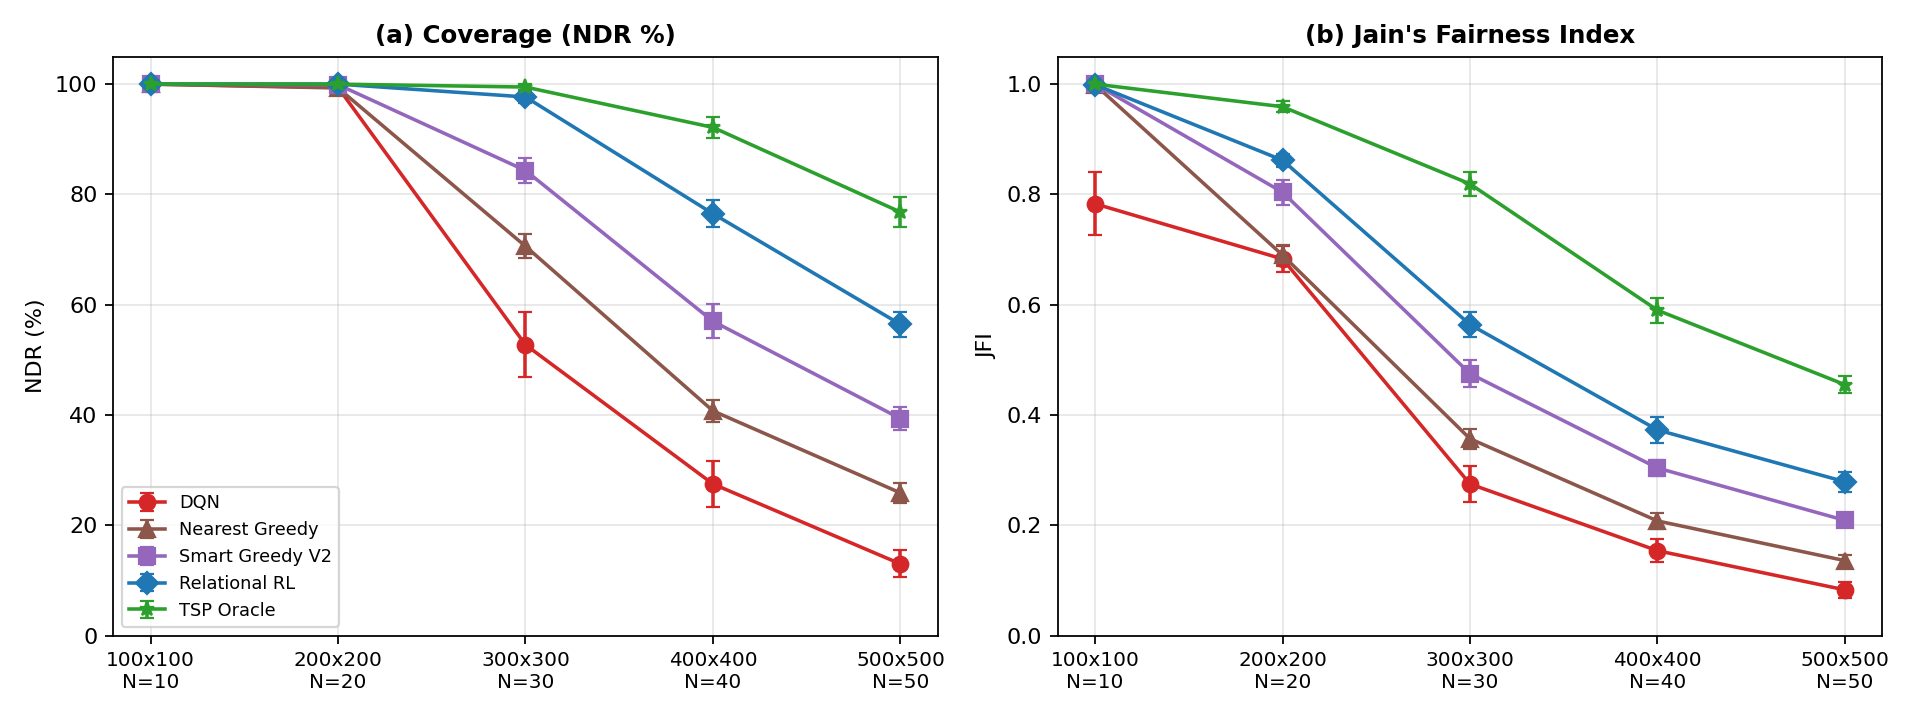
\includegraphics[width=\linewidth]{../src/agents/dqn/dqn_evaluation_results/baseline_results/scalability_combined.png}
\caption{Scalability across five (grid size, $N$) conditions, 50 seeds
per condition. (a) Sensor-coverage (NDR \%). (b) Jain's fairness
index. Error bars are 95\% CIs. Relational RL dominates the DQN and
both greedy baselines at every condition beyond the trivial
$100{\times}100$, and closes a measurable fraction of the TSP-Oracle
ceiling.}
\label{fig:scalability_combined}
\end{figure}

\begin{table}[H]
\centering
\caption{Mean NDR (\%) and Jain's fairness index by agent and condition
(50 seeds / condition; $p$-values from Welch's $t$-test, DQN vs Relational RL).}
\label{tab:scalability_ndr}
\small
\begin{tabularx}{\textwidth}{l X X X X X l}
\toprule
\textbf{Condition} & \textbf{DQN} & \textbf{Nearest} & \textbf{SF-Greedy} & \textbf{Relational RL} & \textbf{TSP Oracle} & $p$ (DQN vs RL) \\
\midrule
$100{\times}100$, $N{=}10$ & 100.0 / 0.78 & 100.0 / 1.00 & 100.0 / 1.00 & 100.0 / 1.00 & 100.0 / 1.00 & N/A \\
$200{\times}200$, $N{=}20$ & 99.4 / 0.68  & 99.3 / 0.69  & 99.9  / 0.80 & \textbf{100.0} / 0.86 & 100.0 / 0.96 & $0.032$ \\
$300{\times}300$, $N{=}30$ & 52.7 / 0.28  & 70.6 / 0.36  & 84.3  / 0.48 & \textbf{97.7} / 0.56  & 99.5 / 0.82 & $<$\,$10^{-4}$ \\
$400{\times}400$, $N{=}40$ & 27.5 / 0.15  & 40.8 / 0.21  & 57.0  / 0.30 & \textbf{76.5} / 0.37  & 92.2 / 0.59 & $<$\,$10^{-4}$ \\
$500{\times}500$, $N{=}50$ & 13.0 / 0.08  & 25.9 / 0.14  & 39.4  / 0.21 & \textbf{56.4} / 0.28  & 76.8 / 0.46 & $<$\,$10^{-4}$ \\
\bottomrule
\end{tabularx}
\end{table}

At $100{\times}100$ all agents saturate at $100\%$ NDR; small fairness differences here just reflect per-sensor collection ratios when any routing strategy can visit every sensor within the episode budget. Past that point the gap grows with scale: Relational RL leads the DQN by $+0.6$ pp at $200{\times}200$ ($p=0.032$), then $+45.0$, $+49.0$, $+43.4$ pp at the three larger conditions (all $p<10^{-4}$). The margin is widest at exactly the conditions where the boundary-occupancy diagnostic predicted the flat-MLP ceiling would bind. The architecture also reverses the earlier result where greedy baselines beat the DQN: at $300{\times}300$, Relational RL leads SF-Aware Greedy by $13.4$ pp and Nearest Greedy by $27.1$ pp.

Jain's Fairness Index follows the same ordering. At $200{\times}200$, Relational RL reaches $0.86$ vs the DQN's $0.68$; the gap is $0.56$ vs $0.28$ at $300{\times}300$ and $0.28$ vs $0.08$ at $500{\times}500$. The greedy baselines sit between the two learned agents throughout, which points to routing quality, not protocol awareness, as the main driver of large-scale performance. SF-Aware Greedy leads Nearest Greedy ($0.48$ vs $0.36$ at $N{=}30$), so SF-awareness does add something at intermediate scale; it is just not enough to close the gap to Relational RL.

A gap to the TSP-Oracle ceiling persists at every condition beyond $100{\times}100$, reaching $20.4$ pp at $500{\times}500$ ($56.4\%$ vs $76.8\%$). The Oracle has full foreknowledge of sensor positions and solves offline; even so it leaves $23.2\%$ of sensors uncollected at $N{=}50$, so the energy budget is genuinely binding rather than a failure of the policy. Relational RL closes $63\%$ of the DQN-to-Oracle gap at $N{=}30$, $58\%$ at $N{=}40$, and $52\%$ at $N{=}50$.

\paragraph{Algorithm vs architecture decomposition.}
Table~\ref{tab:arch_algo_decomp} uses two controlled comparisons to separate algorithm from architecture. In the first, the encoder stays fixed (flat MLP) and only the training algorithm changes: DQN $\to$ PPO adds $+6.2$ pp NDR at $N{=}30$, $+15.0$ pp at $N{=}40$, $+11.7$ pp at $N{=}50$. In the second, the algorithm stays fixed (PPO) and only the encoder changes: flat MLP $\to$ relational adds $+37.7$ pp, $+39.7$ pp, $+33.7$ pp at those conditions. The encoder change accounts for roughly three times the algorithm's contribution at every large-scale condition. Jain's fairness index follows: PPO+Flat-MLP moves the index by at most $0.01$ over the DQN at $N{\ge}30$, while the relational encoder nearly doubles it.

\begin{table}[H]
\centering
\caption{Algorithm $\times$ architecture decomposition: NDR (\%) and Jain's fairness index (mean $\pm$ 95\% CI, $n{=}50$ seeds per condition). DQN vs PPO+Flat-MLP holds architecture fixed; PPO+Flat-MLP vs PPO+Relational holds algorithm fixed.}
\label{tab:arch_algo_decomp}
\small
\begin{tabularx}{\textwidth}{l X X X}
\toprule
\textbf{Condition} & \textbf{DQN (flat MLP)} & \textbf{PPO (flat MLP)} & \textbf{PPO (relational)} \\
\midrule
$100{\times}100$, $N{=}10$ & 100.0\,/\,0.78 & $100.0{\pm}0.0$\,/\,$0.997{\pm}0.001$ & $100.0{\pm}0.0$\,/\,$0.998{\pm}0.000$ \\
$200{\times}200$, $N{=}20$ & 99.4\,/\,0.68  & $98.6{\pm}0.6$\,/\,$0.674{\pm}0.004$  & $100.0{\pm}0.0$\,/\,$0.889{\pm}0.005$ \\
$300{\times}300$, $N{=}30$ & 52.7\,/\,0.28  & $58.9{\pm}1.2$\,/\,$0.264{\pm}0.002$  & $96.6{\pm}0.6$\,/\,$0.589{\pm}0.010$  \\
$400{\times}400$, $N{=}40$ & 27.5\,/\,0.15  & $42.5{\pm}0.9$\,/\,$0.235{\pm}0.002$  & $82.2{\pm}1.1$\,/\,$0.417{\pm}0.004$  \\
$500{\times}500$, $N{=}50$ & 13.0\,/\,0.08  & $24.7{\pm}0.6$\,/\,$0.156{\pm}0.001$  & $58.4{\pm}0.8$\,/\,$0.319{\pm}0.007$  \\
\bottomrule
\end{tabularx}
\end{table}

\paragraph{Energy efficiency.}
Table~\ref{tab:energy_efficiency} adds a third metric to the comparison: bytes collected per watt-hour of battery consumed. At $N{=}10$ the spread is small. At $N{=}20$ the DQN leads PPO+Flat-MLP ($129$ vs $103$\,B/Wh) because the perimeter is a reasonable route when sensors are dense enough to be boundary-adjacent. Beyond $N{=}30$ that ceases to hold. The DQN's efficiency collapses to $10.0$\,B/Wh at $N{=}50$: it burns almost its full battery on perimeter flight and collects almost nothing. PPO+Flat-MLP fares better at $60.1$\,B/Wh but still covers less than a third of sensors at that condition. The relational encoder reaches $136.6$\,B/Wh, $2.3{\times}$ ahead of PPO+Flat-MLP and $13.7{\times}$ ahead of the DQN. The same inductive bias that improves coverage also improves how efficiently the UAV converts flight energy into collected data.

\begin{table}[H]
\centering
\caption{Energy efficiency (bytes per Wh) by agent and condition (mean $\pm$ 95\% CI, $n{=}50$ seeds per condition).}
\label{tab:energy_efficiency}
\small
\begin{tabularx}{\textwidth}{l X X X}
\toprule
\textbf{Condition} & \textbf{DQN (flat MLP)} & \textbf{PPO (flat MLP)} & \textbf{PPO (relational)} \\
\midrule
$100{\times}100$, $N{=}10$ & $91.1{\pm}8.5$   & $138.5{\pm}1.2$ & $130.7{\pm}0.7$ \\
$200{\times}200$, $N{=}20$ & $129.2{\pm}7.0$  & $102.9{\pm}0.8$ & $185.8{\pm}1.9$ \\
$300{\times}300$, $N{=}30$ & $51.8{\pm}14.0$  & $72.9{\pm}0.8$  & $\mathbf{164.3{\pm}2.9}$ \\
$400{\times}400$, $N{=}40$ & $37.8{\pm}12.2$  & $73.7{\pm}0.6$  & $\mathbf{153.5{\pm}1.6}$ \\
$500{\times}500$, $N{=}50$ & $10.0{\pm}5.3$   & $60.1{\pm}0.5$  & $\mathbf{136.6{\pm}2.8}$ \\
\bottomrule
\end{tabularx}
\end{table}
